\documentclass{standalone}
\usepackage{tikz}
\usetikzlibrary{patterns, positioning}
\usetikzlibrary{shapes.misc}
\usepackage[outline]{contour}
\contourlength{1.5pt} 
\usepackage[sfdefault]{ClearSans} %% option 'sfdefault' activates Clear Sans as the default text font
\usepackage[T1]{fontenc}

\begin{document}
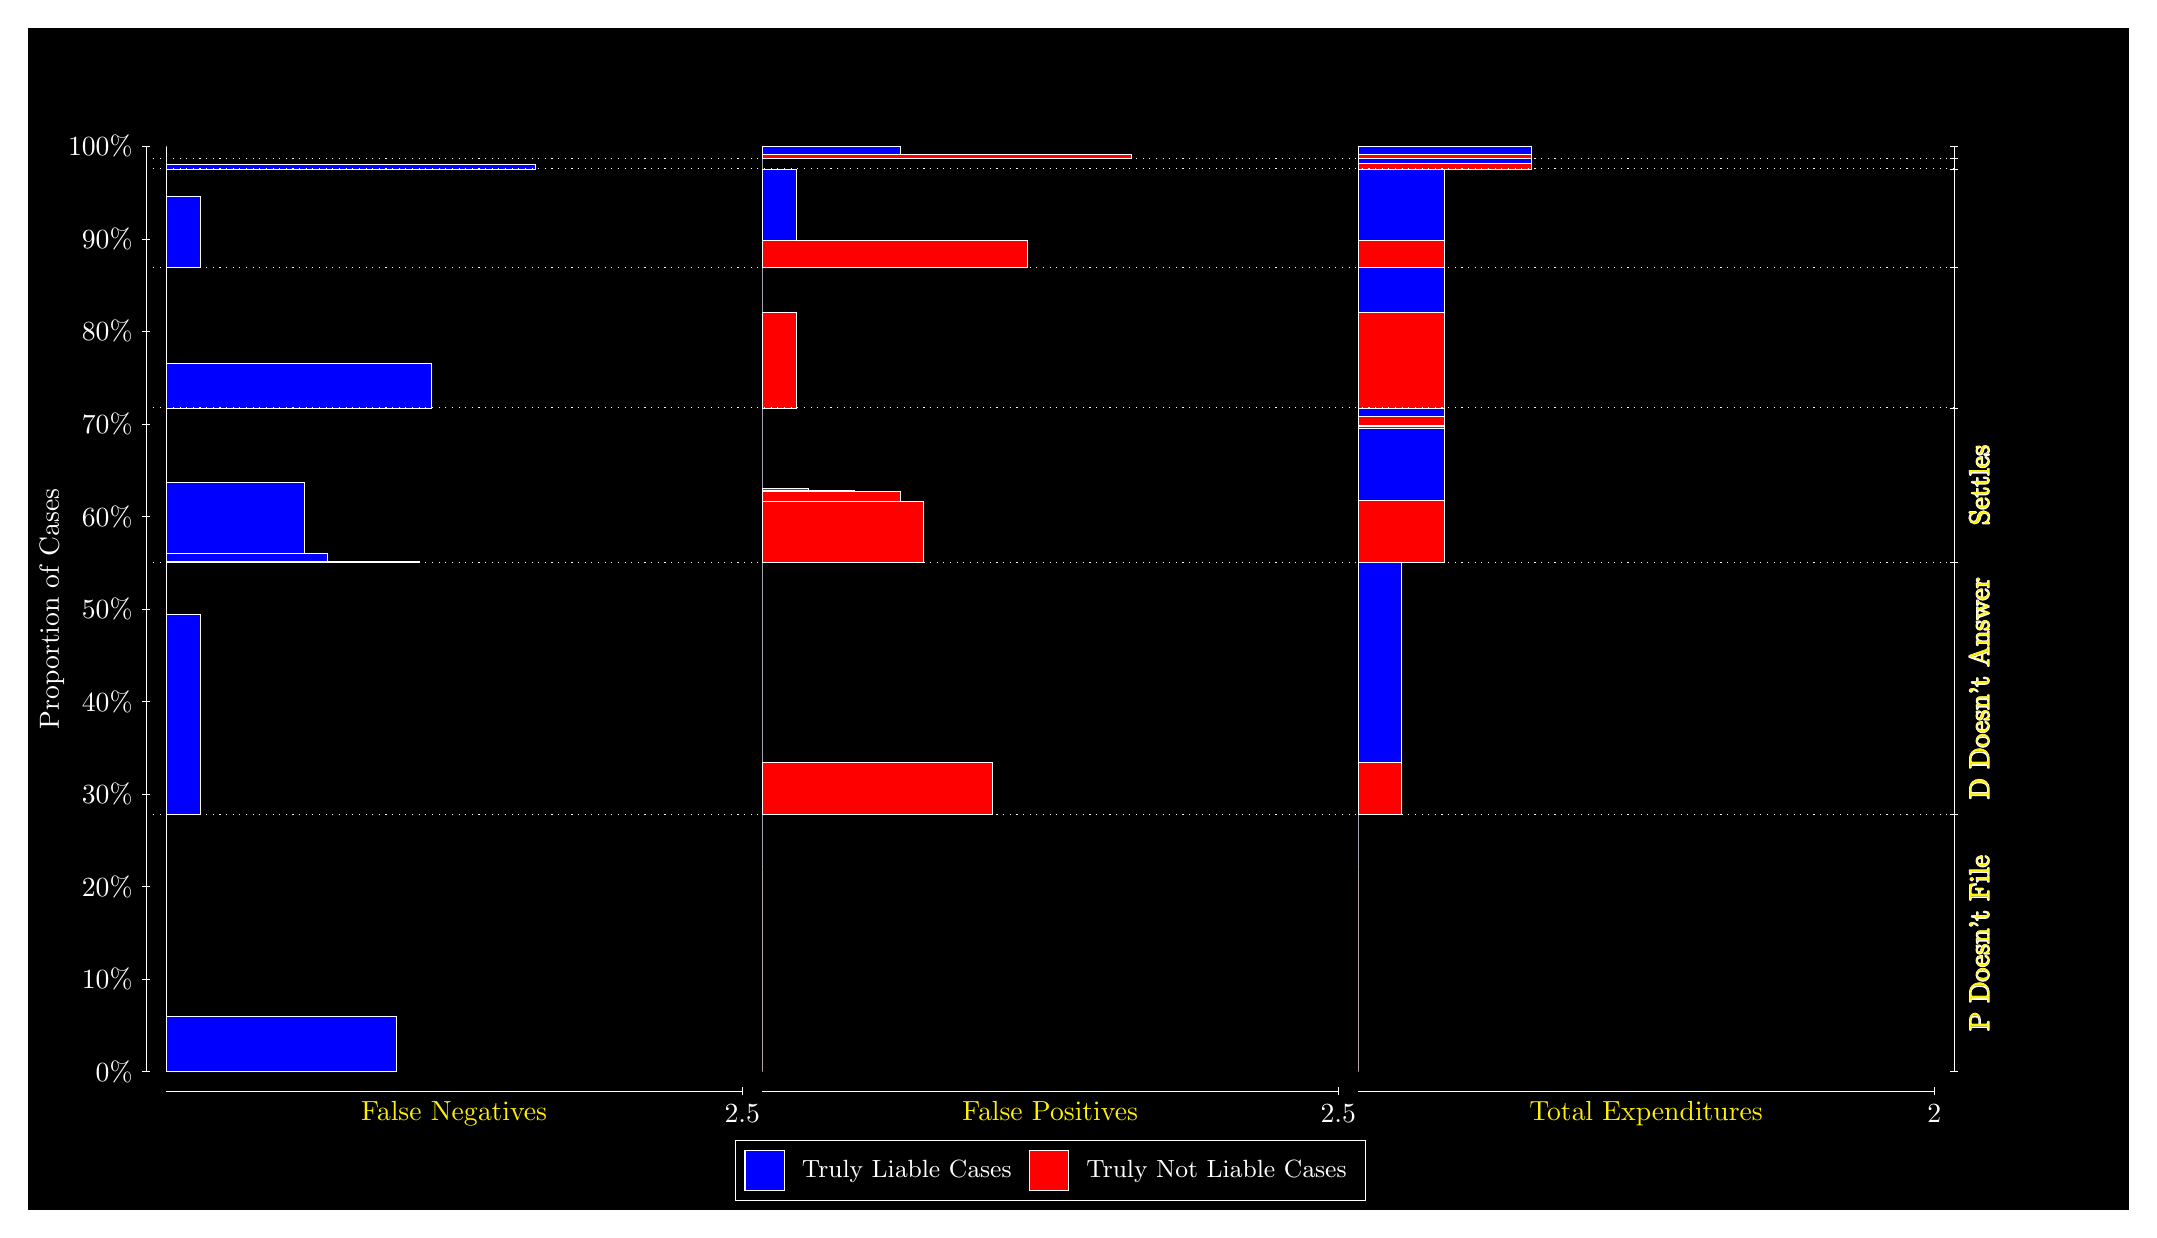
\begin{tikzpicture}
\draw[fill=black] (0,0) rectangle (26.667,15);
\draw[white, very thin] (1.5,1.75) -- (1.5,13.5);
\node[rotate=90, text=white, anchor=center] at (0.3, 7.625) {Proportion of Cases};
\draw[white, very thin] (1.45,1.75) -- (1.55,1.75);
\node[text=white, anchor=east] at (1.45, 1.75) {0\%};
\draw[white, very thin] (1.45,2.925) -- (1.55,2.925);
\node[text=white, anchor=east] at (1.45, 2.925) {10\%};
\draw[white, very thin] (1.45,4.1) -- (1.55,4.1);
\node[text=white, anchor=east] at (1.45, 4.1) {20\%};
\draw[white, very thin] (1.45,5.275) -- (1.55,5.275);
\node[text=white, anchor=east] at (1.45, 5.275) {30\%};
\draw[white, very thin] (1.45,6.45) -- (1.55,6.45);
\node[text=white, anchor=east] at (1.45, 6.45) {40\%};
\draw[white, very thin] (1.45,7.625) -- (1.55,7.625);
\node[text=white, anchor=east] at (1.45, 7.625) {50\%};
\draw[white, very thin] (1.45,8.8) -- (1.55,8.8);
\node[text=white, anchor=east] at (1.45, 8.8) {60\%};
\draw[white, very thin] (1.45,9.975) -- (1.55,9.975);
\node[text=white, anchor=east] at (1.45, 9.975) {70\%};
\draw[white, very thin] (1.45,11.15) -- (1.55,11.15);
\node[text=white, anchor=east] at (1.45, 11.15) {80\%};
\draw[white, very thin] (1.45,12.325) -- (1.55,12.325);
\node[text=white, anchor=east] at (1.45, 12.325) {90\%};
\draw[white, very thin] (1.45,13.5) -- (1.55,13.5);
\node[text=white, anchor=east] at (1.45, 13.5) {100\%};

\draw[white, very thin] (24.457,1.75) -- (24.457,13.5);
\draw[white, very thin] (24.407,1.75) -- (24.507,1.75);
\node[anchor=west] at (24.407, 1.75) {};
\draw[white, very thin] (24.407,5.0144) -- (24.507,5.0144);
\node[anchor=west] at (24.407, 5.0144) {};
\draw[white, very thin] (24.407,8.2188) -- (24.507,8.2188);
\node[anchor=west] at (24.407, 8.2188) {};
\draw[white, very thin] (24.407,10.179) -- (24.507,10.179);
\node[anchor=west] at (24.407, 10.179) {};
\draw[white, very thin] (24.407,11.959) -- (24.507,11.959);
\node[anchor=west] at (24.407, 11.959) {};
\draw[white, very thin] (24.407,13.214) -- (24.507,13.214);
\node[anchor=west] at (24.407, 13.214) {};
\draw[white, very thin] (24.407,13.344) -- (24.507,13.344);
\node[anchor=west] at (24.407, 13.344) {};
\draw[white, very thin] (24.407,13.5) -- (24.507,13.5);
\node[anchor=west] at (24.407, 13.5) {};

\draw[white, very thin, fill=blue] (1.75,1.75) rectangle (4.6775,2.4459);
\draw[white, very thin, fill=red] (1.75,2.4459) rectangle (1.75,5.0144);
\draw[white, very thin, fill=blue] (1.75,5.0144) rectangle (2.1891,7.5524);
\draw[white, very thin, fill=red] (1.75,7.5524) rectangle (1.75,8.2188);
\draw[white, very thin, fill=blue] (1.75,8.2188) rectangle (4.9703,8.2259);
\draw[white, very thin, fill=blue] (1.75,8.2259) rectangle (4.3848,8.2316);
\draw[white, very thin, fill=blue] (1.75,8.2316) rectangle (3.7993,8.3344);
\draw[white, very thin, fill=blue] (1.75,8.3344) rectangle (3.5065,9.2382);
\draw[white, very thin, fill=red] (1.75,9.2382) rectangle (1.75,10.179);
\draw[white, very thin, fill=blue] (1.75,10.179) rectangle (5.1167,10.743);
\draw[white, very thin, fill=red] (1.75,10.743) rectangle (1.75,11.959);
\draw[white, very thin, fill=blue] (1.75,11.959) rectangle (2.1891,12.865);
\draw[white, very thin, fill=red] (1.75,12.865) rectangle (1.75,13.214);
\draw[white, very thin, fill=blue] (1.75,13.214) rectangle (6.4341,13.27);
\draw[white, very thin, fill=red] (1.75,13.27) rectangle (1.75,13.344);
\draw[white, very thin, fill=red] (1.75,13.344) rectangle (1.75,13.405);
\draw[white, very thin, fill=blue] (1.75,13.405) rectangle (1.75,13.5);
\draw[white, very thin, fill=red] (9.3189,1.75) rectangle (9.3189,4.3185);
\draw[white, very thin, fill=blue] (9.3189,4.3185) rectangle (9.3189,5.0144);
\draw[white, very thin, fill=red] (9.3189,5.0144) rectangle (12.246,5.6807);
\draw[white, very thin, fill=blue] (9.3189,5.6807) rectangle (9.3189,8.2188);
\draw[white, very thin, fill=red] (9.3189,8.2188) rectangle (11.368,8.998);
\draw[white, very thin, fill=red] (9.3189,8.998) rectangle (11.075,9.1199);
\draw[white, very thin, fill=red] (9.3189,9.1199) rectangle (10.49,9.1312);
\draw[white, very thin, fill=red] (9.3189,9.1312) rectangle (9.9044,9.1599);
\draw[white, very thin, fill=blue] (9.3189,9.1599) rectangle (9.3189,10.179);
\draw[white, very thin, fill=red] (9.3189,10.179) rectangle (9.758,11.396);
\draw[white, very thin, fill=blue] (9.3189,11.396) rectangle (9.3189,11.959);
\draw[white, very thin, fill=red] (9.3189,11.959) rectangle (12.686,12.308);
\draw[white, very thin, fill=blue] (9.3189,12.308) rectangle (9.758,13.214);
\draw[white, very thin, fill=red] (9.3189,13.214) rectangle (9.3189,13.288);
\draw[white, very thin, fill=blue] (9.3189,13.288) rectangle (9.3189,13.344);
\draw[white, very thin, fill=red] (9.3189,13.344) rectangle (14.003,13.405);
\draw[white, very thin, fill=blue] (9.3189,13.405) rectangle (11.075,13.5);
\draw[white, very thin, fill=red] (16.888,1.75) rectangle (16.888,4.3185);
\draw[white, very thin, fill=blue] (16.888,4.3185) rectangle (16.888,5.0144);
\draw[white, very thin, fill=red] (16.888,5.0144) rectangle (17.437,5.6807);
\draw[white, very thin, fill=blue] (16.888,5.6807) rectangle (17.437,8.2188);
\draw[white, very thin, fill=red] (16.888,8.2188) rectangle (17.986,9.0093);
\draw[white, very thin, fill=blue] (16.888,9.0093) rectangle (17.986,9.9187);
\draw[white, very thin, fill=red] (16.888,9.9187) rectangle (17.986,9.9474);
\draw[white, very thin, fill=blue] (16.888,9.9474) rectangle (17.986,9.9545);
\draw[white, very thin, fill=red] (16.888,9.9545) rectangle (17.986,10.076);
\draw[white, very thin, fill=blue] (16.888,10.076) rectangle (17.986,10.179);
\draw[white, very thin, fill=red] (16.888,10.179) rectangle (17.986,11.396);
\draw[white, very thin, fill=blue] (16.888,11.396) rectangle (17.986,11.959);
\draw[white, very thin, fill=red] (16.888,11.959) rectangle (17.986,12.308);
\draw[white, very thin, fill=blue] (16.888,12.308) rectangle (17.986,13.214);
\draw[white, very thin, fill=red] (16.888,13.214) rectangle (19.083,13.288);
\draw[white, very thin, fill=blue] (16.888,13.288) rectangle (19.083,13.344);
\draw[white, very thin, fill=red] (16.888,13.344) rectangle (19.083,13.405);
\draw[white, very thin, fill=blue] (16.888,13.405) rectangle (19.083,13.5);
\draw[white, dotted] (1.5,5.0144) -- (24.457,5.0144);
\draw[white, dotted] (1.5,8.2188) -- (24.457,8.2188);
\draw[white, dotted] (1.5,10.179) -- (24.457,10.179);
\draw[white, dotted] (1.5,11.959) -- (24.457,11.959);
\draw[white, dotted] (1.5,13.214) -- (24.457,13.214);
\draw[white, dotted] (1.5,13.344) -- (24.457,13.344);
\draw[white, very thin] (1.75,1.5) -- (9.0689,1.5);
\node[text=yellow, anchor=north] at (5.4094, 1.5) {False Negatives};
\draw[white, very thin] (9.0689,1.45) -- (9.0689,1.55);
\node[text=white, anchor=north] at (9.0689, 1.45) {2.5};

\draw[white, very thin] (9.3189,1.5) -- (16.638,1.5);
\node[text=yellow, anchor=north] at (12.978, 1.5) {False Positives};
\draw[white, very thin] (16.638,1.45) -- (16.638,1.55);
\node[text=white, anchor=north] at (16.638, 1.45) {2.5};

\draw[white, very thin] (16.888,1.5) -- (24.207,1.5);
\node[text=yellow, anchor=north] at (20.547, 1.5) {Total Expenditures};
\draw[white, very thin] (24.207,1.45) -- (24.207,1.55);
\node[text=white, anchor=north] at (24.207, 1.45) {2};

\node[text=yellow, centered, rotate=90] at (24.777, 3.3822) {\contour{white}{P Doesn't File}};
\node[text=yellow, centered, rotate=90] at (24.777, 6.6166) {\contour{white}{D Doesn't Answer}};
\node[text=yellow, centered, rotate=90] at (24.777, 9.199) {\contour{white}{Settles}};





\draw (12.978300999999998,1.5) node[draw=none] (baseCoordinate) {};
\begin{scope}[align=center]
        \matrix[scale=0.5, draw=white, below=0.5cm of baseCoordinate, nodes={draw}, column sep=0.1cm]{
            \node[rectangle, draw, minimum width=0.5cm, minimum height=0.5cm, fill=blue] {}; &
            \node[draw=none, font=\small, text=white] (B) {Truly Liable Cases}; &
            \node[rectangle, draw, minimum width=0.5cm, minimum height=0.5cm, fill=red] {}; &
            \node[draw=none, font=\small, text=white] (B) {Truly Not Liable Cases}; \\
            };
\end{scope}

\end{tikzpicture}
\end{document}